\documentclass[11pt, a4paper, onecolumn, confidential, copyright]{hawkfranklin}

\usepackage[utf8]{inputenc}
\usepackage[T1]{fontenc}
\usepackage{graphicx}
\usepackage{float}
\usepackage{amsmath,amssymb}
\usepackage{url}
\usepackage{booktabs}
\usepackage{longtable}
\usepackage{array}
\usepackage{enumitem}
\usepackage[numbers,super,sort&compress]{natbib}
\usepackage[dvipsnames]{xcolor}
\usepackage{placeins}
\usepackage{hyperref}
\setlength{\emergencystretch}{3em}

\captionsetup[figure]{font=footnotesize}
\captionsetup[table]{font=footnotesize}
\renewcommand{\absfont}{\normalfont\linespread{1.2}\fontsize{9}{11}\selectfont}
\hypersetup{colorlinks=true,linkcolor=Blue,citecolor=Green,urlcolor=NavyBlue}
\bibliographystyle{abbrvnat}

\keywords{tabular foundation models; cancer multiomics; survival classification; cohort effects; missingness; evaluation design}
\paperurl{https://github.com/HawkFranklin-Research/tab-r1}
\title{From Predictive Gains to Cohort Shortcuts: Stress-Testing Tabular Foundation Models in Cancer Multiomics}
\correspondingauthor{evaluator@hawk-franklin-research.com}
\reportnumber{TR-2026-09-02}
\renewcommand{\today}{2026-09-02}

\author[1]{Vatsal P. Patel\textsuperscript{*}}
\affil[1]{HawkFranklin Research, India}
\affil[ ]{\textsuperscript{*}Corresponding author: \href{mailto:evaluator@hawk-franklin-research.com}{evaluator@hawk-franklin-research.com}}

\begin{abstract}
\noindent\textbf{Background:} Tabular foundation models offer in-context prediction without task-specific parameter fitting, but their behavior in high-dimensional biomedical data remains difficult to separate from cohort structure and evaluation design. Cancer multiomics provides a stringent test because molecular measurements, outcome prevalence, data source, and missingness patterns vary across disease cohorts.

\noindent\textbf{Methods:} We evaluated five classical learners, AutoGluon, TabFM, and four TabPFN generations on 400 frozen patient-grouped folds spanning breast, esophageal, head and neck, lung squamous, and lung adenocarcinoma cohorts. Outcomes were 3-year and 5-year overall-survival event classification and an exploratory extreme-survival contrast. Each task used five repeats of five-fold evaluation, validation-only threshold selection, and molecular feature selection confined to the training partition. We compared within-cancer and randomly pooled evaluation and examined cancer-identity, structural-zero, label-permutation, and cancer-held-out diagnostics.

\noindent\textbf{Results:} Mean within-cancer ROC AUC for the foundation models ranged from 0.563 to 0.568, indicating modest and heterogeneous discrimination. Pooled ROC AUC increased to 0.714--0.721 for evaluated 3-year configurations, 0.751--0.754 for 5-year survival, and 0.778--0.786 for the extreme contrast. Cancer identity alone reached ROC AUC values of 0.707, 0.703, and 0.809 across the three endpoints, while structural-zero patterns reached 0.745, 0.704, and 0.824. A cancer-held-out linear molecular diagnostic remained near chance, with mean ROC AUC values of 0.479, 0.508, and 0.518.

\noindent\textbf{Conclusions:} Foundation models were competitive with strong tree ensembles, but no architecture dominated consistently. The increase produced by random pan-cancer pooling cannot be interpreted as evidence of a shared prognostic molecular signature because cohort identity and harmonization structure carried comparable predictive information. Biomedical evaluations of tabular foundation models should report within-cohort results, explicit shortcut controls, and cohort-aware generalization tests alongside pooled scores.
\end{abstract}

\begin{document}
\maketitle

\section{Introduction}
\label{sec:introduction}

Structured data remain central to biomedical research, yet predictive modeling on tables differs from modeling text or images. Feature scales, missingness mechanisms, sample sizes, and semantic relations between columns can change substantially from one dataset to another. Gradient-boosted trees and related ensembles remain difficult to displace under these conditions because they capture nonlinear interactions, tolerate mixed feature distributions, and can be tuned effectively within realistic compute budgets. XGBoost, LightGBM, CatBoost, random forests, and AutoGluon therefore provide necessary comparators for any claim that a foundation model has changed the practical state of tabular learning.\citep{breiman2001random,chen2016xgboost,ke2017lightgbm,prokhorenkova2018catboost,erickson2020autogluon,grinsztajn2022tree}

Tabular foundation models approach the problem differently. Prior-fitted networks learn an inference procedure during pretraining and then condition on labeled examples at prediction time. TabPFN demonstrated that this strategy can provide strong small-data classification performance without conventional task-specific optimization.\citep{hollmann2025accurate} More recent TabPFN releases extend the supported data regime and inference system, while TabICL investigates in-context learning at larger scale.\citep{qu2025tabicl} TabFM is also an in-context tabular model, but it was trained on synthetic datasets sampled from structural causal models and uses alternating row and column attention with row compression.\citep{google2026tabfm,tabfmsoftware2026} These systems differ in architecture, training distribution, resource requirements, and supported input envelope. Comparisons based only on headline accuracy can therefore conceal consequential differences in probabilistic performance, runtime, and model coverage.

Independent evaluation is especially important because tabular rankings are sensitive to data splits, preprocessing, validation budgets, ensembling, and hardware. TabArena has emphasized the effect of evaluation protocol and time budget on model comparisons, while broad empirical studies continue to find that tree ensembles are strong on medium-sized tabular datasets.\citep{erickson2025tabarena,grinsztajn2022tree} A fair comparison requires identical patient partitions, train-only preprocessing, preserved sample-level predictions, and metrics that assess both discrimination and probability quality. ROC AUC alone is insufficient when outcome prevalence differs across tasks. Precision-recall AUC should be interpreted relative to prevalence, and log loss or Brier score should not be described as evidence of calibration without examining calibration behavior directly.\citep{saito2015precision,van2019calibration,brier1950verification}

Cancer multiomics is a demanding setting for this evaluation. Molecular tables commonly have many more candidate variables than patients, survival outcomes are censored, and cohorts differ in tissue of origin, assay availability, source, and baseline prognosis. These differences are not merely nuisance variation. A pooled model may identify cancer type or data source through expression values, modality availability, or structural zeros and then exploit between-cohort outcome prevalence without learning a molecular mechanism that transfers to a new cohort. Batch-label confounding can produce strongly optimistic cross-validation estimates, and performance can fall sharply under cross-study validation.\citep{soneson2014batch,bernau2014crossstudy,ambroise2002selection} Consequently, higher pooled discrimination is an observation to be explained rather than direct evidence of a pan-cancer prognostic signature.

We used five cancer cohorts to ask four questions. First, under identical frozen folds, how do successive TabPFN models, TabFM, AutoGluon, and classical learners compare in within-cancer survival event classification? Second, how much does random pooling alter apparent discrimination? Third, can cancer identity and structural missingness account for part of that increase? Fourth, does the signal remain under cancer-held-out diagnostics? The study focuses on fixed-horizon event classification rather than full time-to-event modeling or clinical risk stratification. The extreme-survival analysis is treated as a separate exploratory estimand because excluding intermediate outcomes changes both the target population and the difficulty of the task.

\section{Results}
\label{sec:results}

\subsection{Cohort construction exposes endpoint and modality heterogeneity}

The analysis integrated breast invasive carcinoma (BRCA), esophageal carcinoma (ESCA), head and neck squamous cell carcinoma (HNSCC), lung squamous cell carcinoma (LSCC), and lung adenocarcinoma (LUAD) resources derived from TCGA and CPTAC data products (Figure~\ref{fig:cohort_design}).\citep{tcga2012brca,tcga2017esca,tcga2015hnsc,tcga2012lusc,tcga2014luad,liu2018clinical,li2023pancancer} Raw cohort sizes ranged from 182 patients for ESCA to 1,206 for BRCA. Applying fixed-horizon eligibility rules reduced the usable sample count because patients censored before a horizon could not be assigned a valid event label. The 3-year tasks retained 86 to 501 patients per cancer; 5-year and extreme-survival tasks were not formed for ESCA because the eligible cohort did not satisfy the prespecified requirements (Table~\ref{tab:cohorts}).

The resulting study contained 16 cohort-endpoint tasks and 400 frozen folds. Per-cancer tasks contributed 325 folds, comprising five cancers at 3 years and four cancers each for 5-year and extreme survival. Three pooled endpoints contributed a further 75 folds. The pooled 3-year cohort contained 1,645 eligible patients, compared with 1,168 at 5 years and 937 in the extreme contrast. Multiomics feature composition also varied by cohort. This heterogeneity motivated the later shortcut analyses because the pattern of observed and structurally absent modalities could reveal cohort membership independently of survival biology.

\begin{figure}[p]
\centering
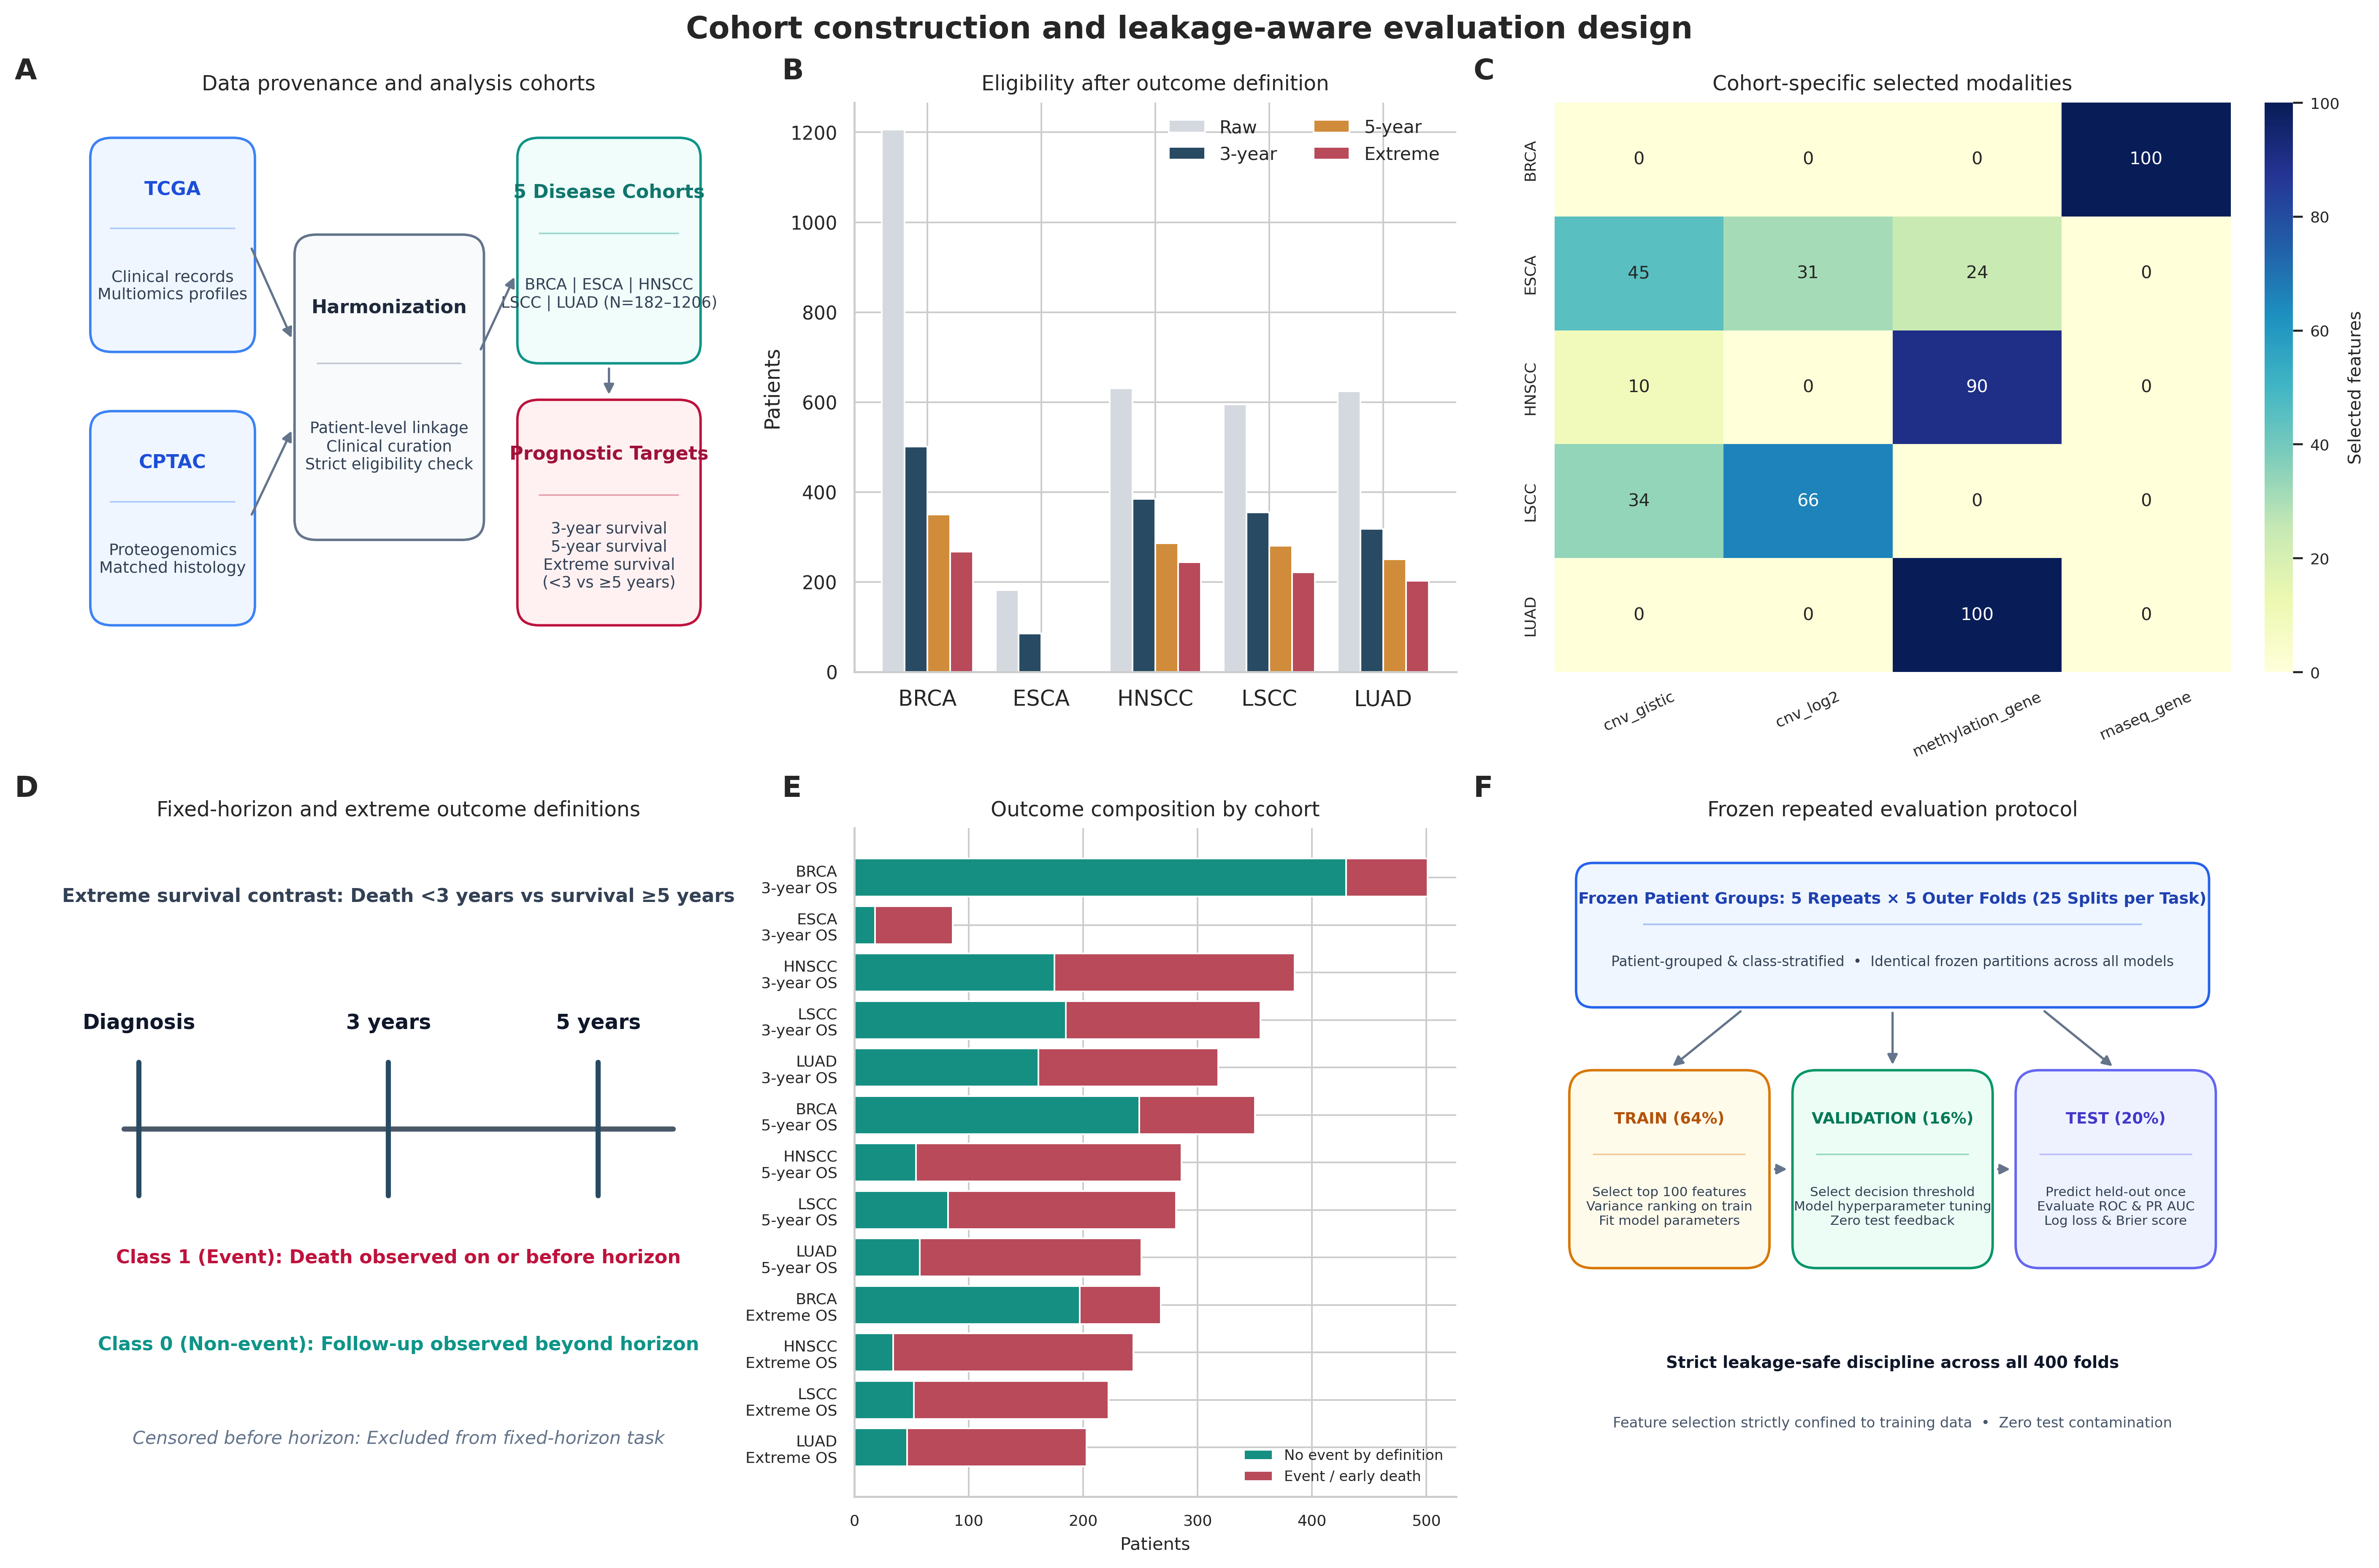
\includegraphics[width=\linewidth]{figures/manuscript/figure_01_cohort_and_design.pdf}
\caption{\textbf{Cohort construction and leakage-safe evaluation design.} \textbf{A}, Provenance and assembly of the five cancer cohorts. \textbf{B}, Raw and endpoint-eligible patient counts. \textbf{C}, Molecular modality composition by cohort. \textbf{D}, Definitions of the 3-year, 5-year, and exploratory extreme-survival targets. \textbf{E}, Class counts and prevalence among eligible patients. \textbf{F}, Five repeats of five-fold patient-grouped evaluation with feature selection fitted on training patients and decision thresholds selected using validation data.}
\label{fig:cohort_design}
\end{figure}

\begin{table}[ht]
\centering
\caption{Cancer cohort size and endpoint eligibility. Extreme survival contrasts death within 3 years against survival beyond 5 years. NA indicates that an endpoint-specific cohort was not formed.}
\label{tab:cohorts}
\begin{tabular}{lrrrr}
\toprule
Cohort & Raw & 3-year eligible & 5-year eligible & Extreme eligible \\
\midrule
BRCA & 1206 & 501 & 350 & 268 \\
ESCA & 182 & 86 & NA & NA \\
HNSCC & 631 & 385 & 286 & 244 \\
LSCC & 595 & 355 & 281 & 222 \\
LUAD & 624 & 318 & 251 & 203 \\
\bottomrule
\end{tabular}

\end{table}

\subsection{Within-cancer discrimination is modest and model rankings are heterogeneous}

Across homogeneous cancer cohorts, the principal result was not a decisive foundation-model victory but a narrow band of modest discrimination (Figure~\ref{fig:within_cancer}). Foundation-model macro-average ROC AUC ranged from 0.563 for TabPFN v3 to 0.568 for TabPFN v2.5. TabFM reached 0.565. Random forest was the strongest classical model by this summary at 0.561, followed by CatBoost at 0.559, while AutoGluon reached 0.550. Differences of this magnitude were smaller than the variation across cancer-endpoint tasks. They therefore do not support designation of a universal winner.

Model behavior also depended on the endpoint. For example, the foundation models generally performed better on the selected extreme-survival populations than on the fixed-horizon tasks, but the same pattern was visible for tree ensembles. Precision-recall performance varied with event prevalence, and several apparently high PR AUC values occurred in tasks with a high positive-class fraction. Figure~\ref{fig:within_cancer} therefore reports PR AUC above the prevalence reference rather than treating raw PR AUC as directly comparable across cohorts. Fold-matched differences from random forest were distributed around small positive and negative values, reinforcing that architecture alone did not determine performance.

\begin{figure}[p]
\centering
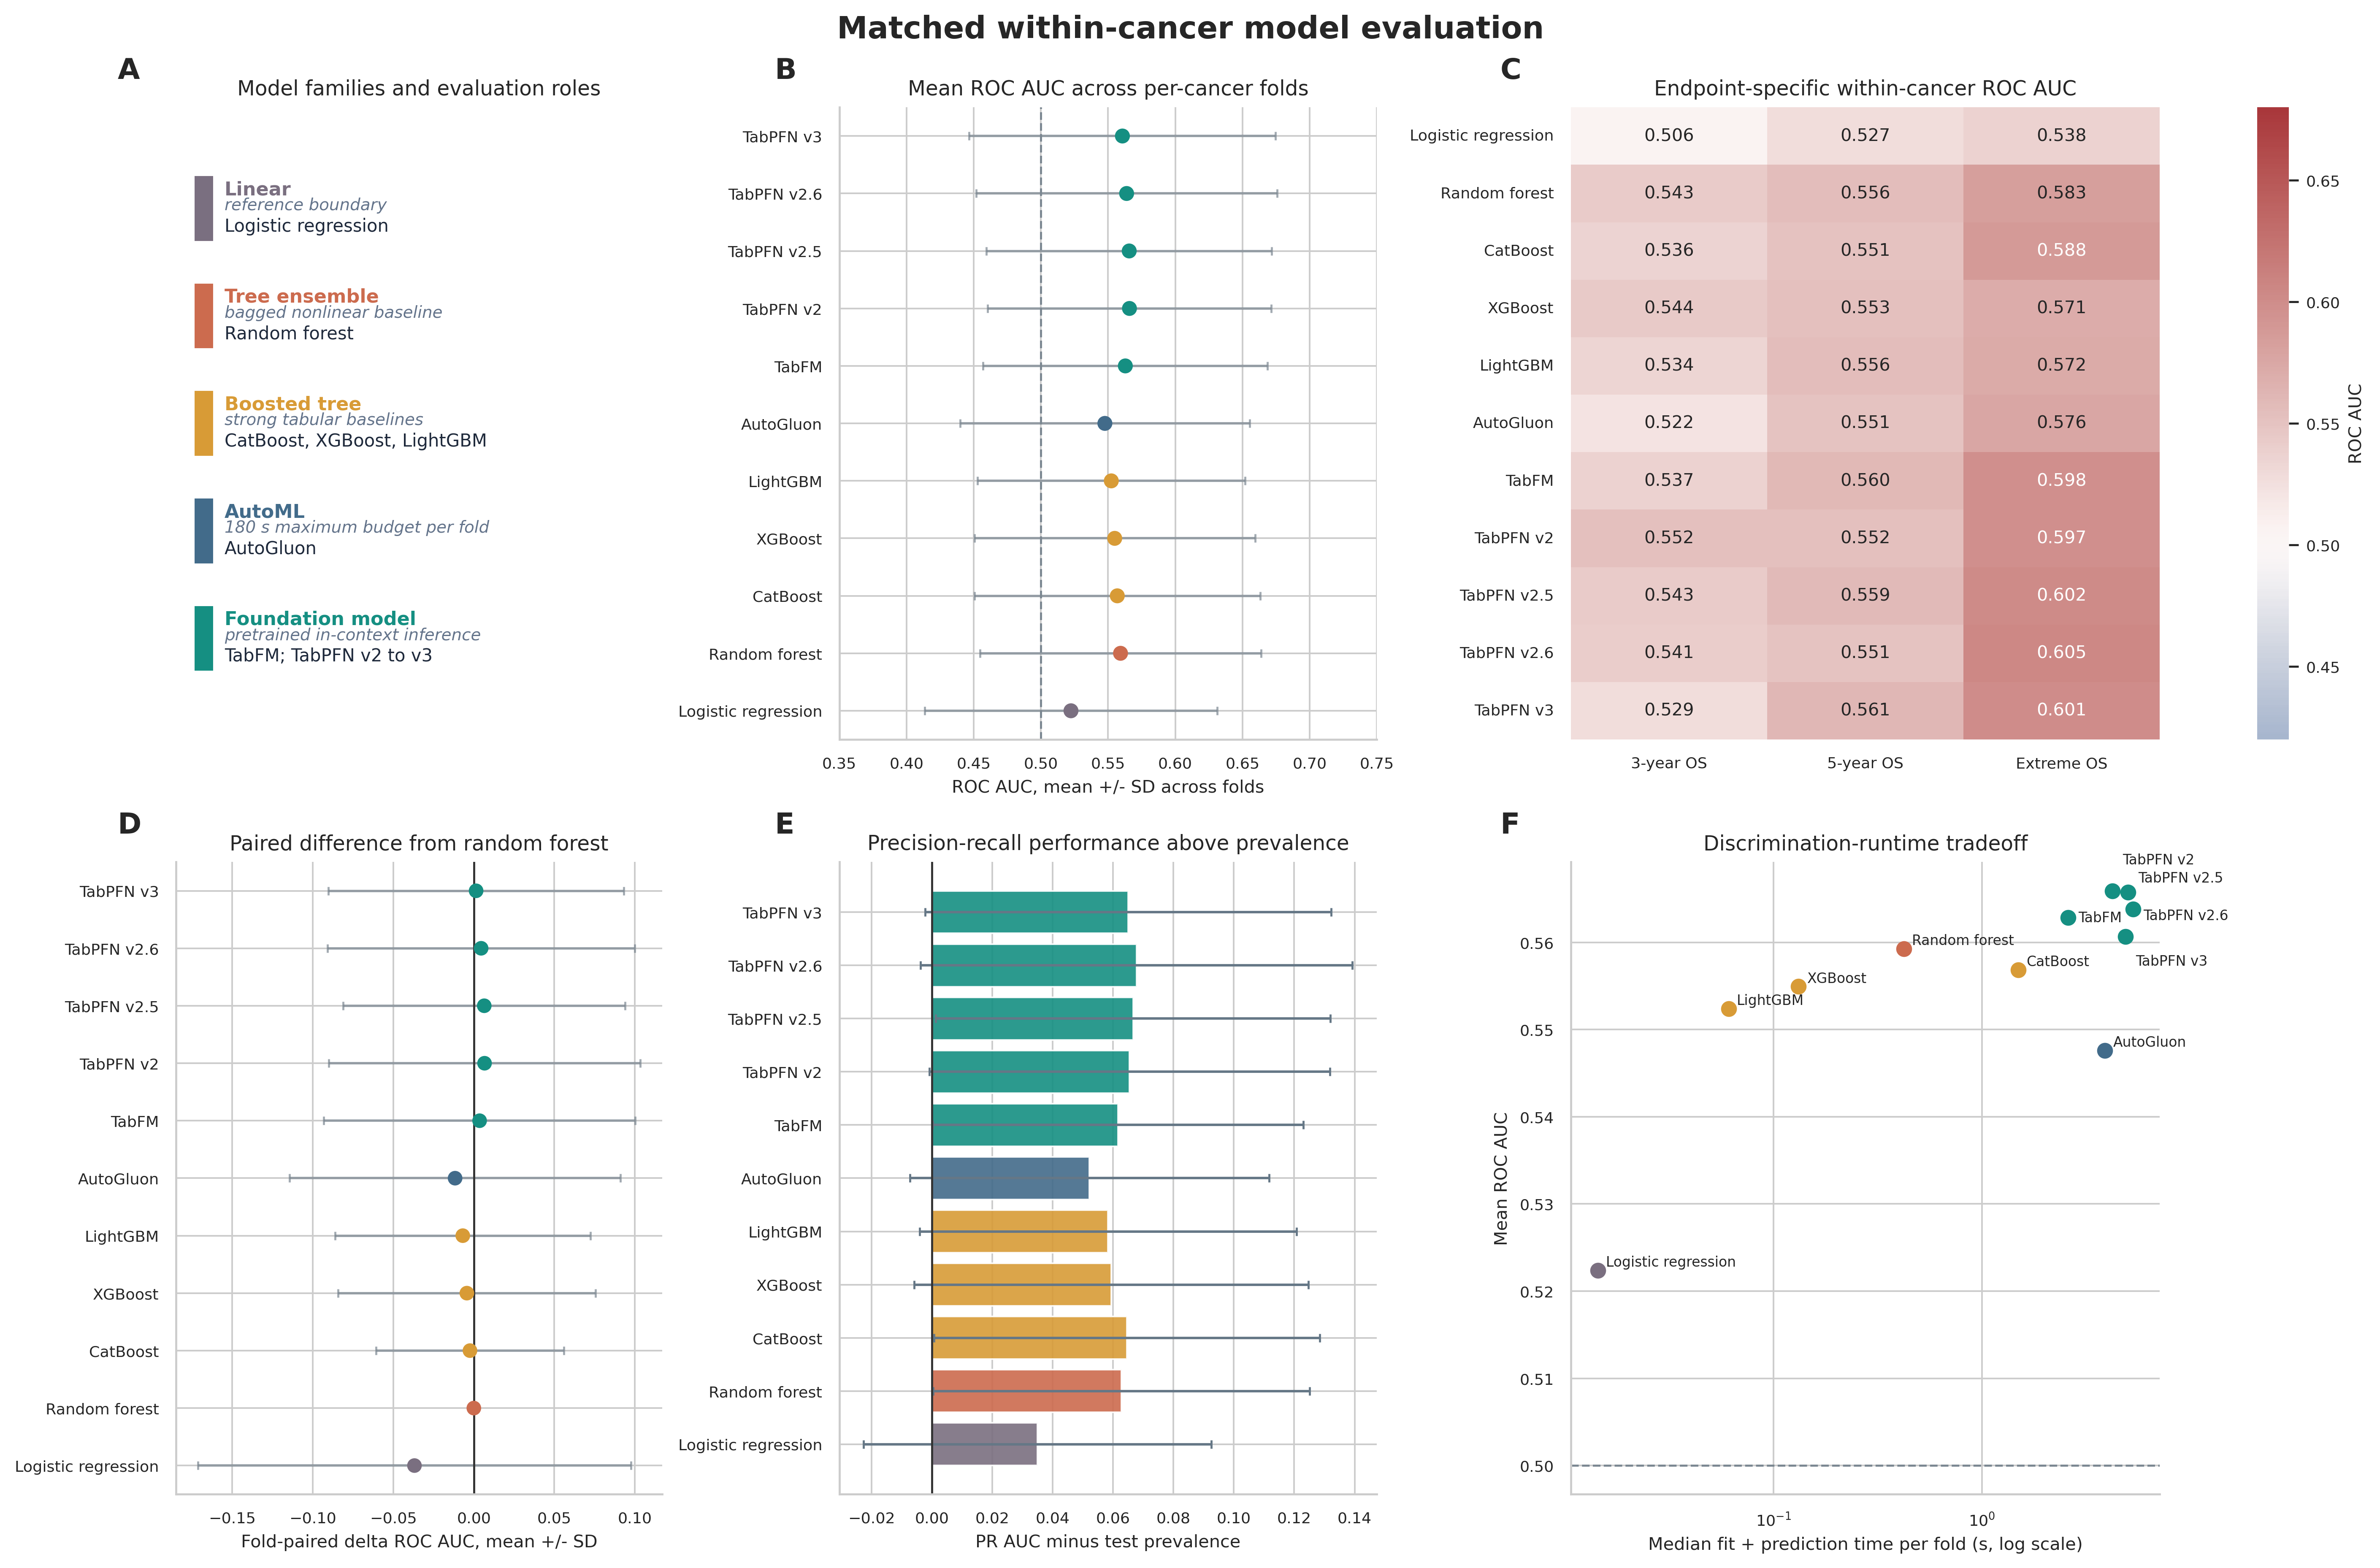
\includegraphics[width=\linewidth]{figures/manuscript/figure_02_within_cancer_performance.pdf}
\caption{\textbf{Matched model performance within cancer cohorts.} \textbf{A}, Evaluated model families and execution paradigms. \textbf{B}, Mean within-cancer ROC AUC with variation across frozen folds. \textbf{C}, ROC AUC by model and endpoint. \textbf{D}, Fold-matched ROC AUC difference relative to random forest. \textbf{E}, precision-recall AUC above endpoint prevalence. \textbf{F}, discrimination and median runtime tradeoff. The figure emphasizes heterogeneity rather than a winner-only ranking.}
\label{fig:within_cancer}
\end{figure}

\subsection{Random pooling increases apparent discrimination across model families}

Pooling cancers increased ROC AUC for nearly every nonlinear model (Figure~\ref{fig:pooling}). Random forest rose from a within-cancer macro-average of 0.561 to 0.716, 0.747, and 0.781 on pooled 3-year, 5-year, and extreme-survival tasks, respectively. TabFM rose from 0.565 to 0.721, 0.753, and 0.780. TabPFN v3 reached 0.714, 0.754, and 0.786. The concordant shift across foundation models, boosted trees, and AutoML indicates that the pooled gain was not specific to one pretrained architecture.

The largest values occurred in the exploratory extreme-survival task. That result should not be interpreted as improvement on the fixed-window estimand. The extreme contrast excluded intermediate outcomes and compared more separated patient groups, reducing the sample from 1,645 eligible patients at 3 years to 937. Pooled performance also concealed variation when predictions were stratified back into constituent cancers. Together, these findings show that adding heterogeneous cohorts made the pooled classification problem easier in aggregate, but do not establish that the learned ranking represented a shared molecular survival mechanism.

\begin{table}[ht]
\centering
\caption{Mean ROC AUC across frozen folds. Within-cancer is the macro-average over the three endpoint summaries. NA denotes a configuration outside the evaluated CPU execution envelope.}
\label{tab:model_auc}
\resizebox{\linewidth}{!}{\begin{tabular}{llrrrr}
\toprule
Model & Family & Within-cancer & Pooled 3-year & Pooled 5-year & Pooled extreme \\
\midrule
Logistic regression & Linear & 0.524 & 0.536 & 0.542 & 0.522 \\
Random forest & Tree ensemble & 0.561 & 0.716 & 0.747 & 0.781 \\
CatBoost & Boosted tree & 0.559 & 0.713 & 0.749 & 0.782 \\
XGBoost & Boosted tree & 0.556 & 0.701 & 0.734 & 0.768 \\
LightGBM & Boosted tree & 0.554 & 0.698 & 0.719 & 0.762 \\
AutoGluon & AutoML & 0.550 & 0.702 & 0.744 & 0.757 \\
TabFM & Foundation model & 0.565 & 0.721 & 0.753 & 0.780 \\
TabPFN v2 & Foundation model & 0.567 & NA & 0.751 & 0.784 \\
TabPFN v2.5 & Foundation model & 0.568 & NA & 0.753 & 0.785 \\
TabPFN v2.6 & Foundation model & 0.566 & NA & 0.752 & 0.778 \\
TabPFN v3 & Foundation model & 0.563 & 0.714 & 0.754 & 0.786 \\
\bottomrule
\end{tabular}
}
\end{table}

\begin{figure}[p]
\centering
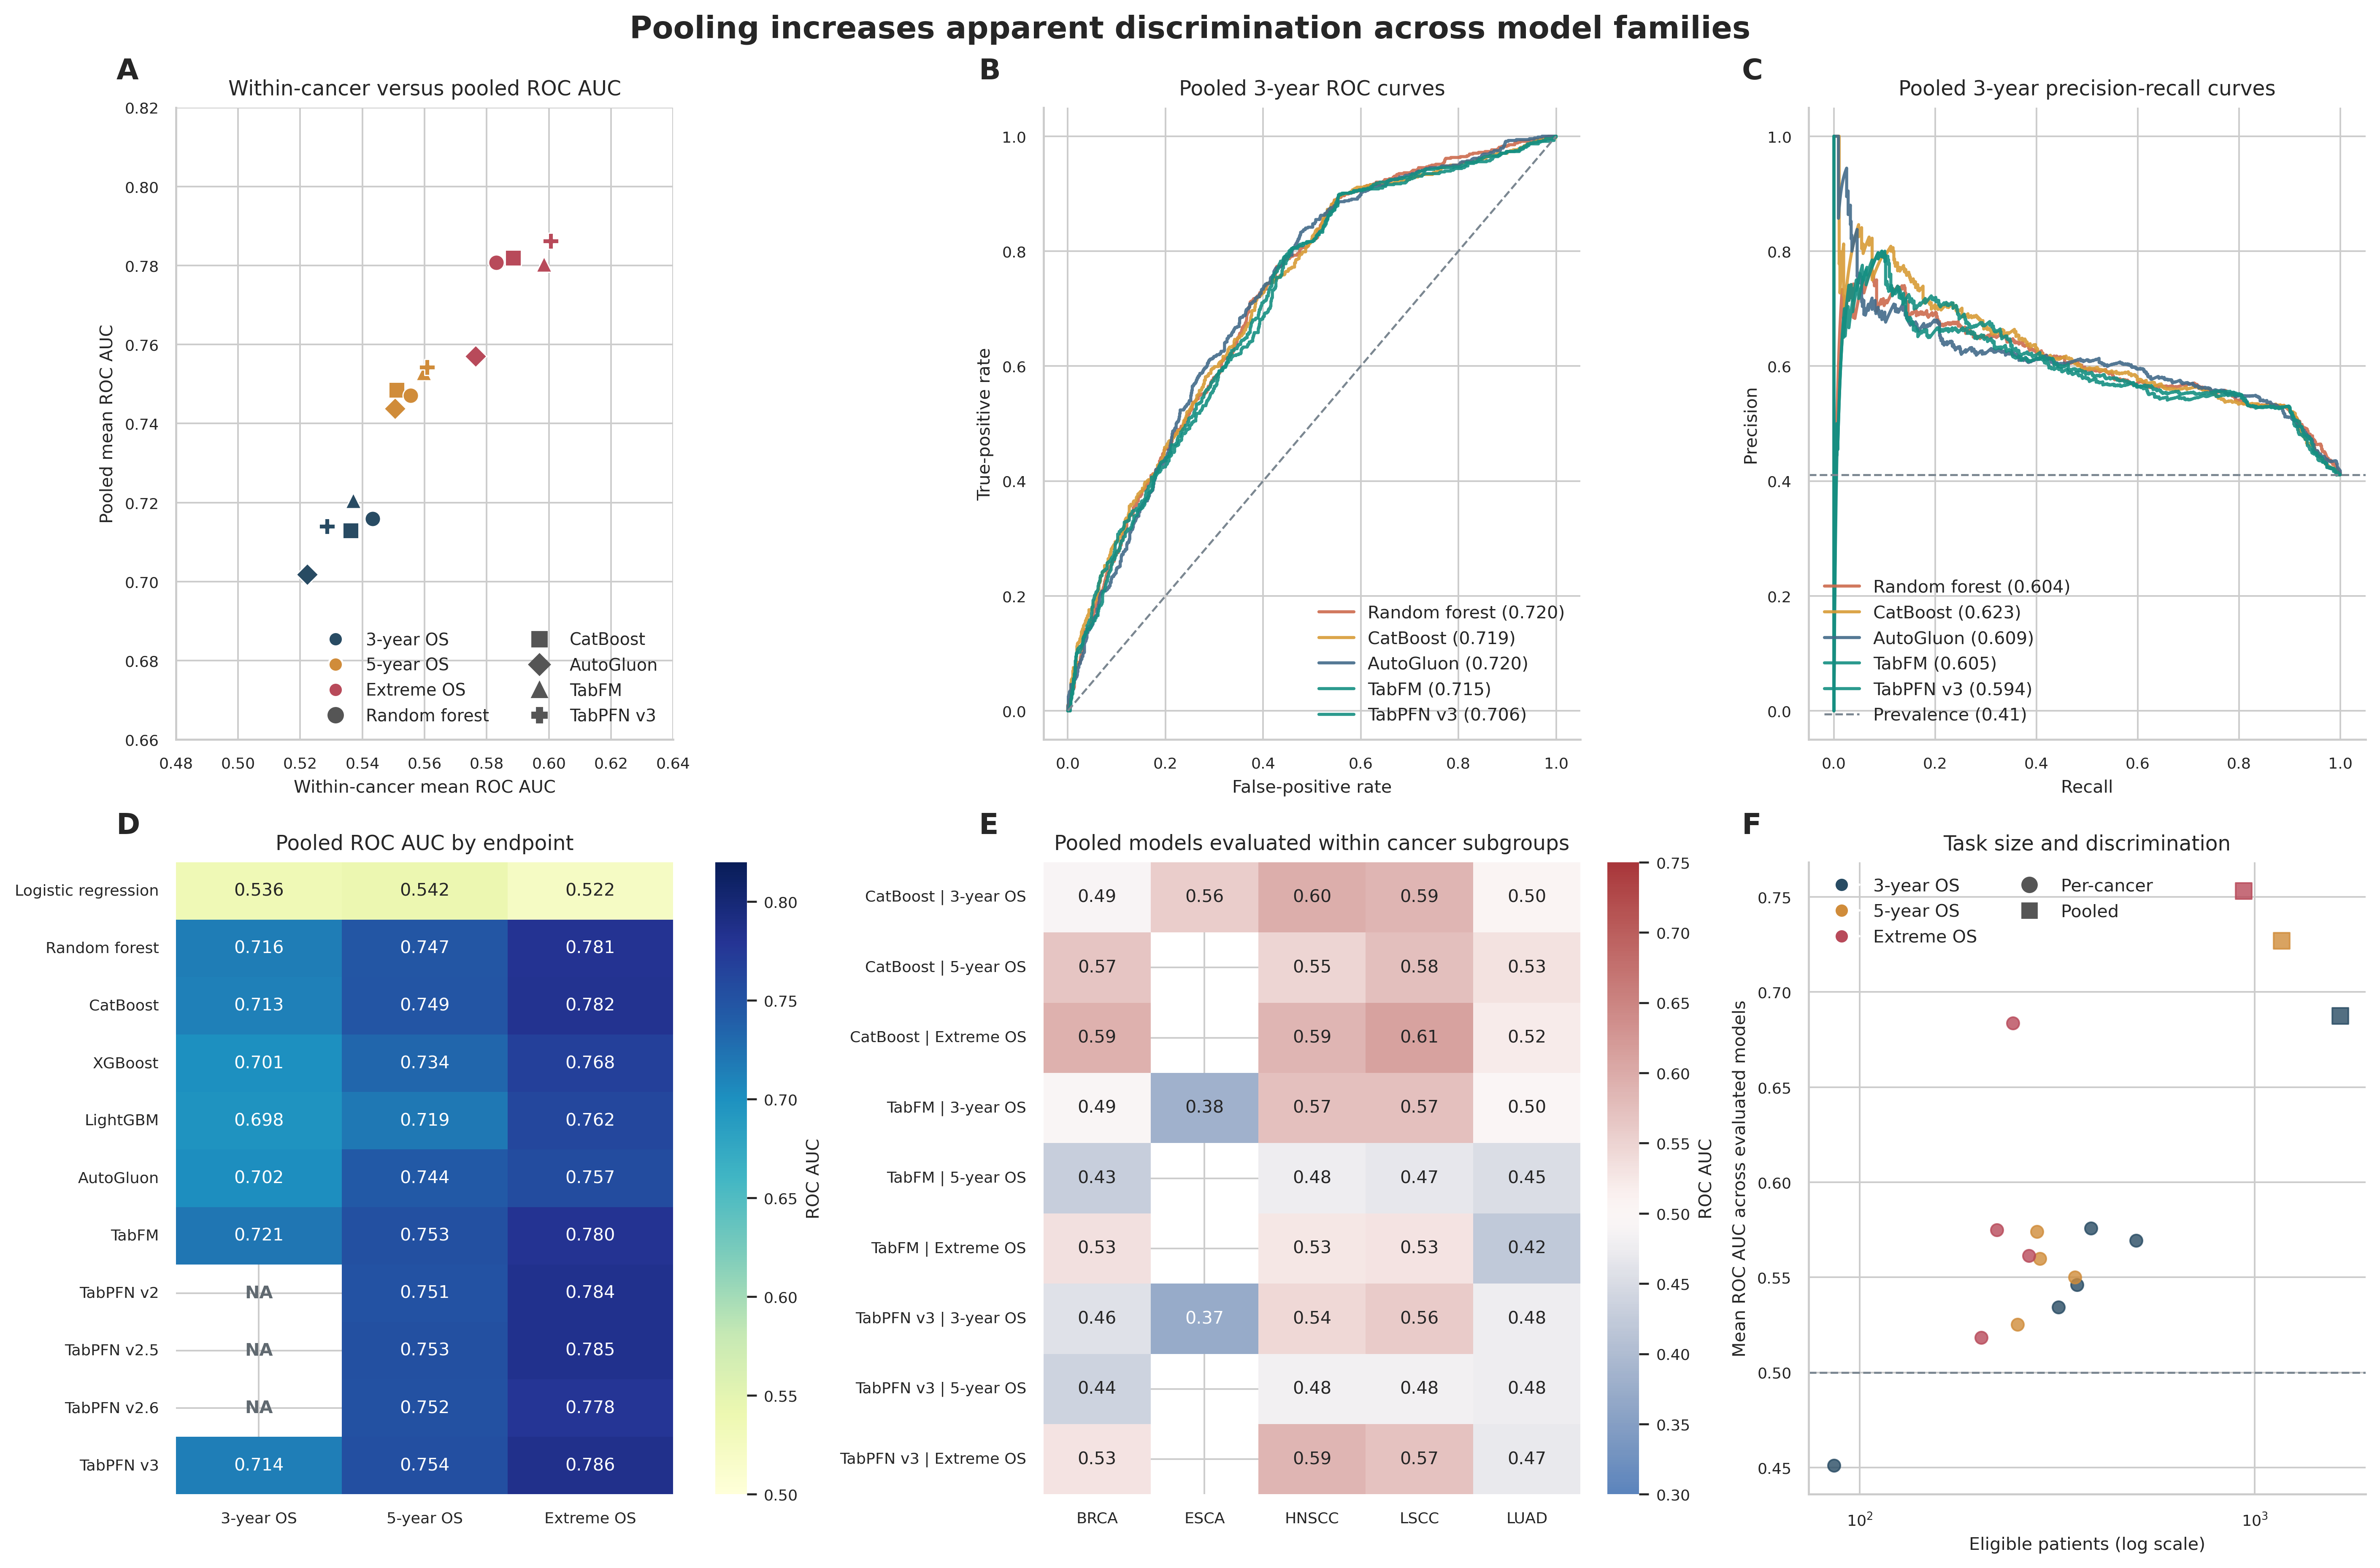
\includegraphics[width=\linewidth]{figures/manuscript/figure_03_pooling_effect.pdf}
\caption{\textbf{Apparent gains from random pan-cancer pooling.} \textbf{A}, Connected within-cancer and pooled ROC AUC summaries. \textbf{B}, Pooled 3-year out-of-fold ROC curves for configurations with available predictions. \textbf{C}, Corresponding precision-recall curves with the prevalence reference. \textbf{D}, Pooled ROC AUC across endpoints; unavailable configurations are marked NA. \textbf{E}, Pooled predictions evaluated within constituent cancers. \textbf{F}, Relationship between task size and discrimination.}
\label{fig:pooling}
\end{figure}

\subsection{Cancer identity and structural missingness account for substantial pooled separability}

Shortcut controls changed the interpretation of the pooled results (Figure~\ref{fig:shortcuts}). A model supplied only cancer identity achieved ROC AUC values of 0.707 for 3-year survival, 0.703 for 5-year survival, and 0.809 for the extreme contrast. A model based on structural-zero patterns reached 0.745, 0.704, and 0.824. For 3-year survival and the extreme contrast, the structural-zero control exceeded the best evaluated molecular model summary. Cancer identity was itself highly recoverable from harmonization structure: structural-zero patterns produced balanced accuracy of approximately 0.985 in cancer classification, whereas a molecular-value diagnostic reached approximately 0.480.

The cancer-held-out linear molecular diagnostic provided a complementary stress test. Mean ROC AUC was 0.479 at 3 years, 0.508 at 5 years, and 0.518 for extreme survival, substantially below the random pooled values. Label-permutation distributions further showed how much performance could arise after disrupting the survival association globally or within cancer. These controls do not prove that every pooled prediction was a shortcut, nor do they quantify a unique causal contribution for each artifact. They do show that cohort-associated information was strong enough to reproduce much of the apparent pooled discrimination and that this signal did not transfer reliably when cancer identity was held out.

\begin{table}[ht]
\centering
\caption{Pooled shortcut and cancer-held-out diagnostics. Values are ROC AUC. The best evaluated molecular model is selected separately for each endpoint.}
\label{tab:shortcuts}
\begin{tabular}{lrrrr}
\toprule
Endpoint & Cancer identity & Structural zero & Best evaluated model & Held-out molecular \\
\midrule
3-year OS & 0.707 & 0.745 & 0.721 & 0.479 \\
5-year OS & 0.703 & 0.704 & 0.754 & 0.508 \\
Extreme OS & 0.809 & 0.824 & 0.786 & 0.518 \\
\bottomrule
\end{tabular}

\end{table}

\begin{figure}[p]
\centering
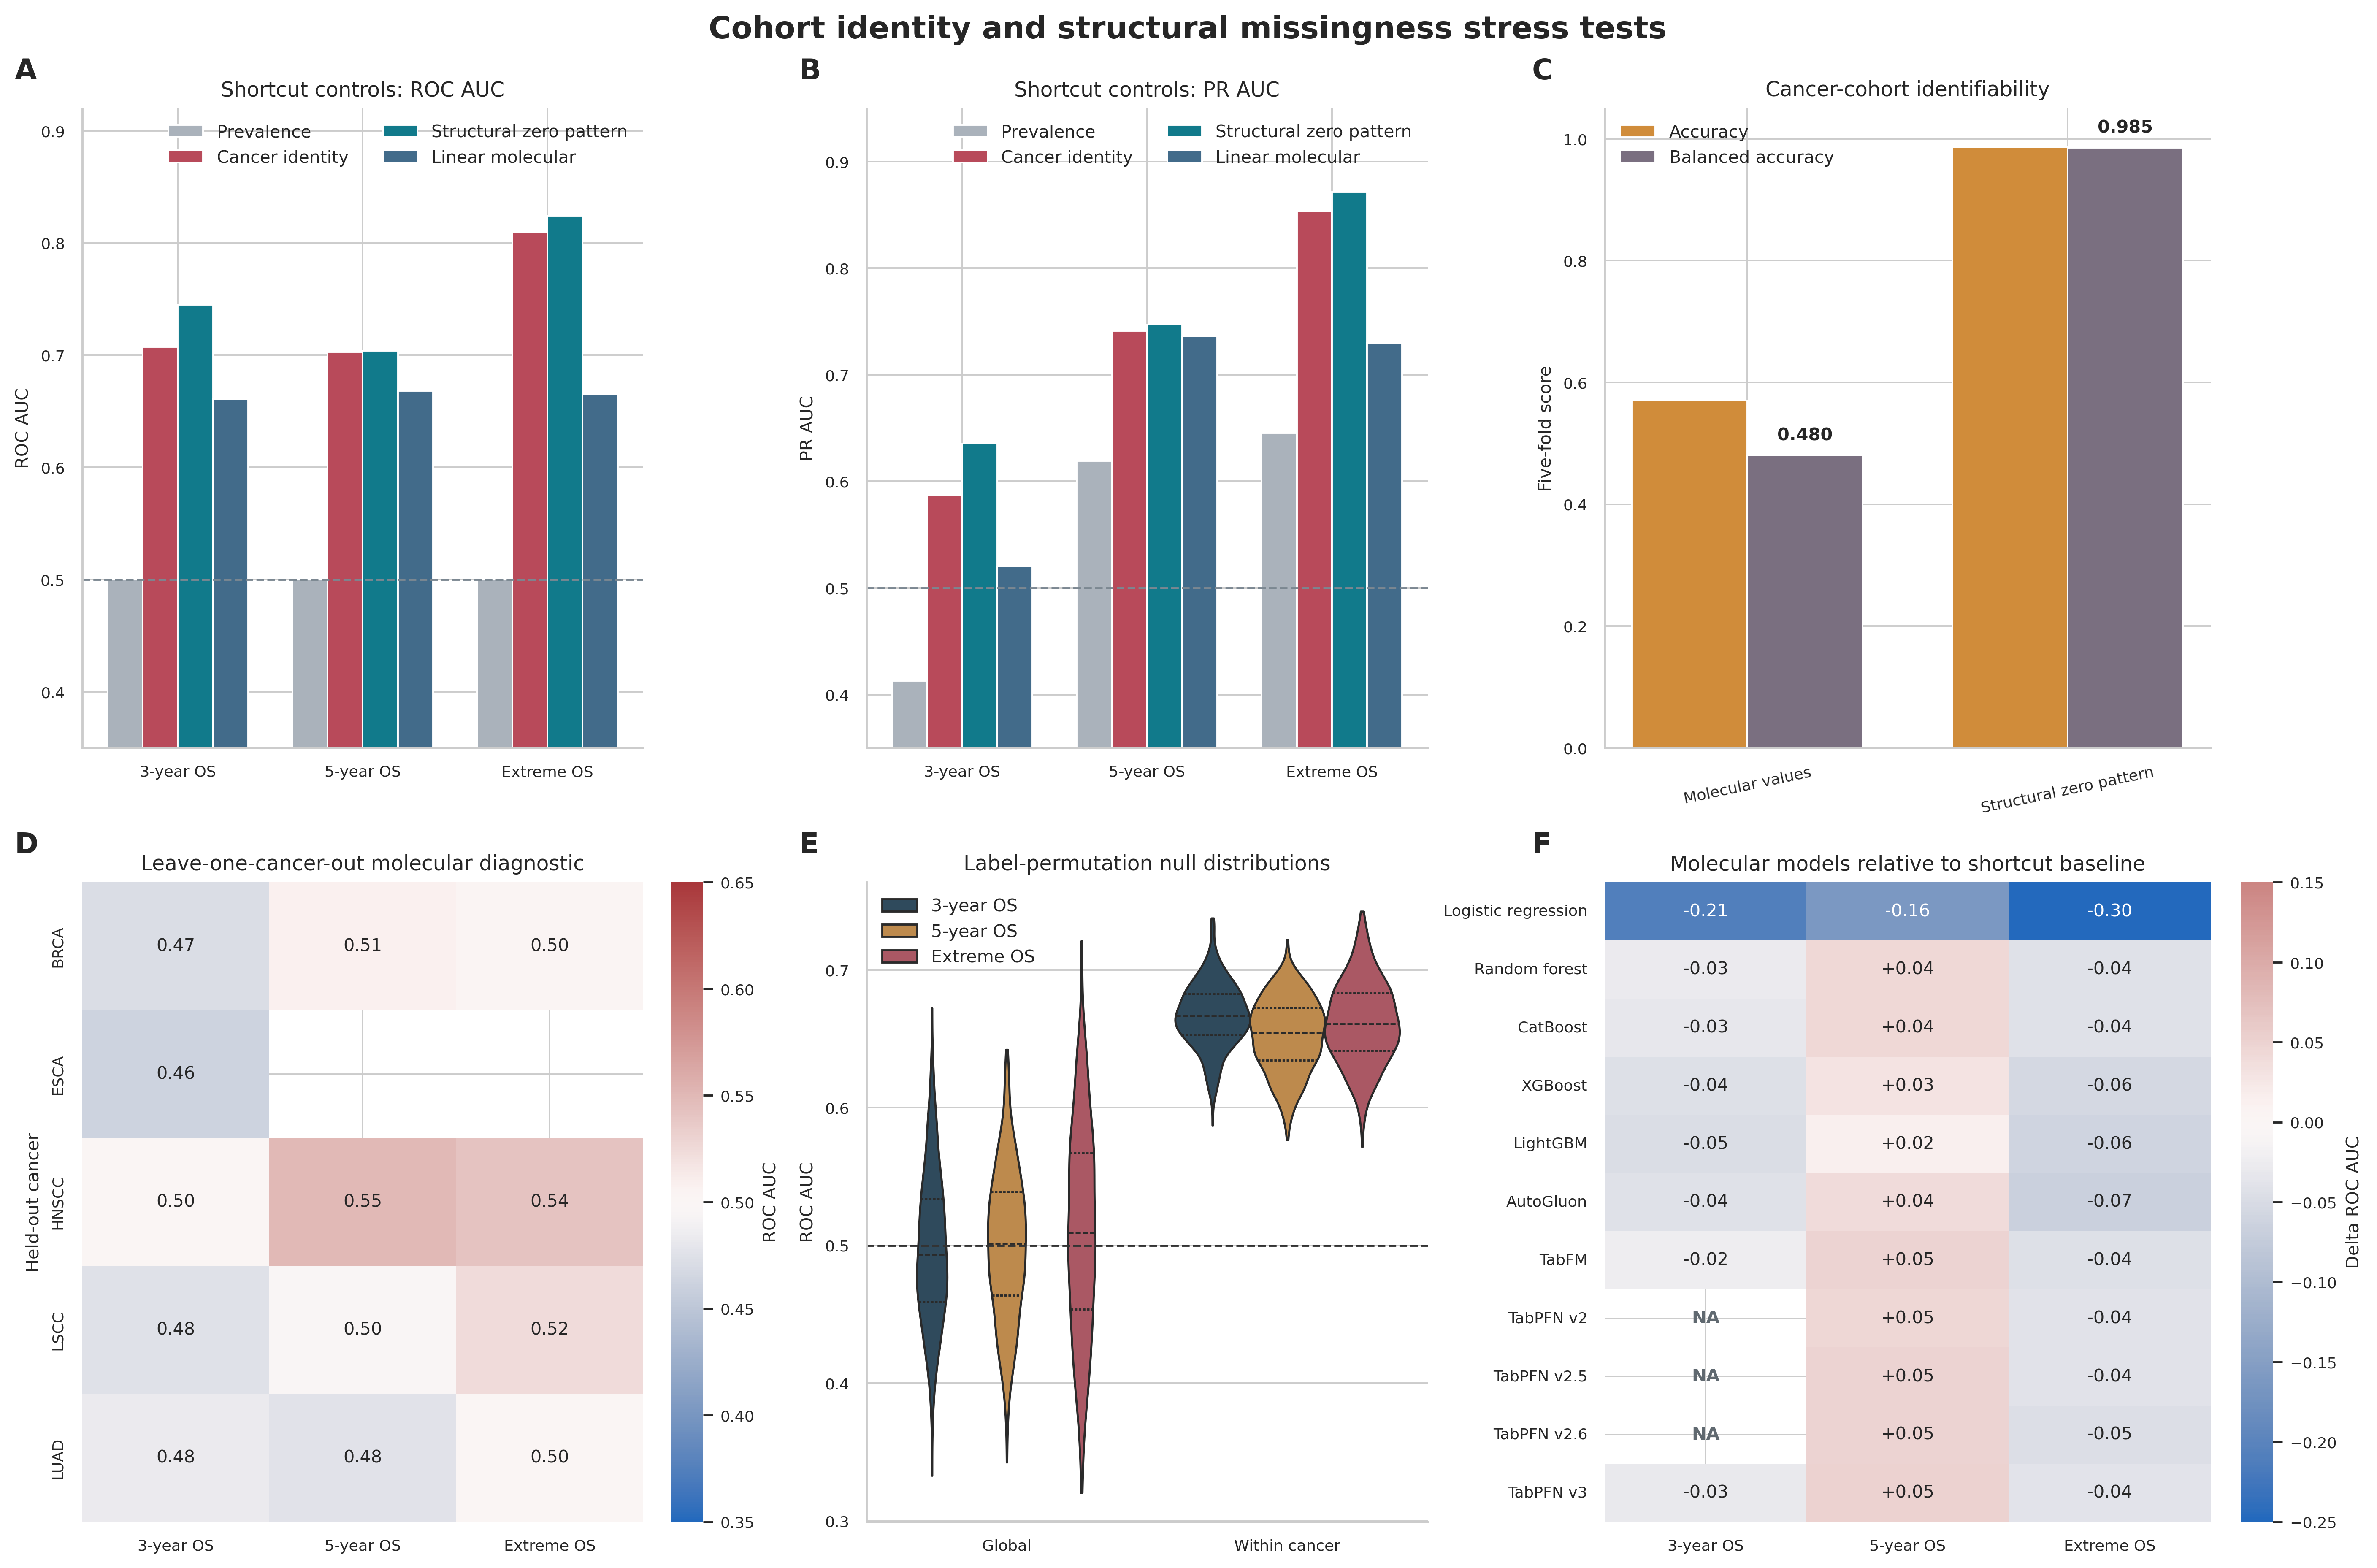
\includegraphics[width=\linewidth]{figures/manuscript/figure_04_shortcut_stress_tests.pdf}
\caption{\textbf{Cohort and missingness shortcut diagnostics.} \textbf{A}, Cancer-identity-only discrimination. \textbf{B}, Structural-zero control performance. \textbf{C}, Cancer-cohort separability from molecular values and zero patterns. \textbf{D}, cancer-held-out linear molecular diagnostics. \textbf{E}, global and within-cancer label-permutation distributions. \textbf{F}, difference between each pooled model and the strongest shortcut control; unavailable configurations are marked NA.}
\label{fig:shortcuts}
\end{figure}

\subsection{Probability quality and compute profiles prevent a single model ordering}

Discrimination did not provide a complete ranking. Brier score and log loss varied by model and endpoint, while calibration curves showed deviations that were not apparent from ROC AUC alone (Figure~\ref{fig:probability_compute}). Operating characteristics also depended on thresholds selected from validation data. Sensitivity and specificity are consequently presented as secondary summaries rather than intrinsic properties of a model. Lower log loss or Brier score indicates better aggregate probabilistic accuracy in this evaluation, but neither metric alone establishes calibration across clinically relevant risk ranges.

Runtime separated the model families more clearly than accuracy. Classical estimators and the in-context systems differed in fit and prediction cost, while AutoGluon used a fixed per-fold search budget. The complete cloud evaluation used CPU execution on a Google Cloud \texttt{c3-highcpu-22} Spot instance. TabFM used its PyTorch backend, and AutoGluon received 180 seconds per fold. These operational differences are part of the comparison because a small numerical gain may not justify a substantially different compute envelope. Complete fold-level metrics and sample-level predictions were retained to permit later recalculation without rerunning the models.

\begin{figure}[p]
\centering
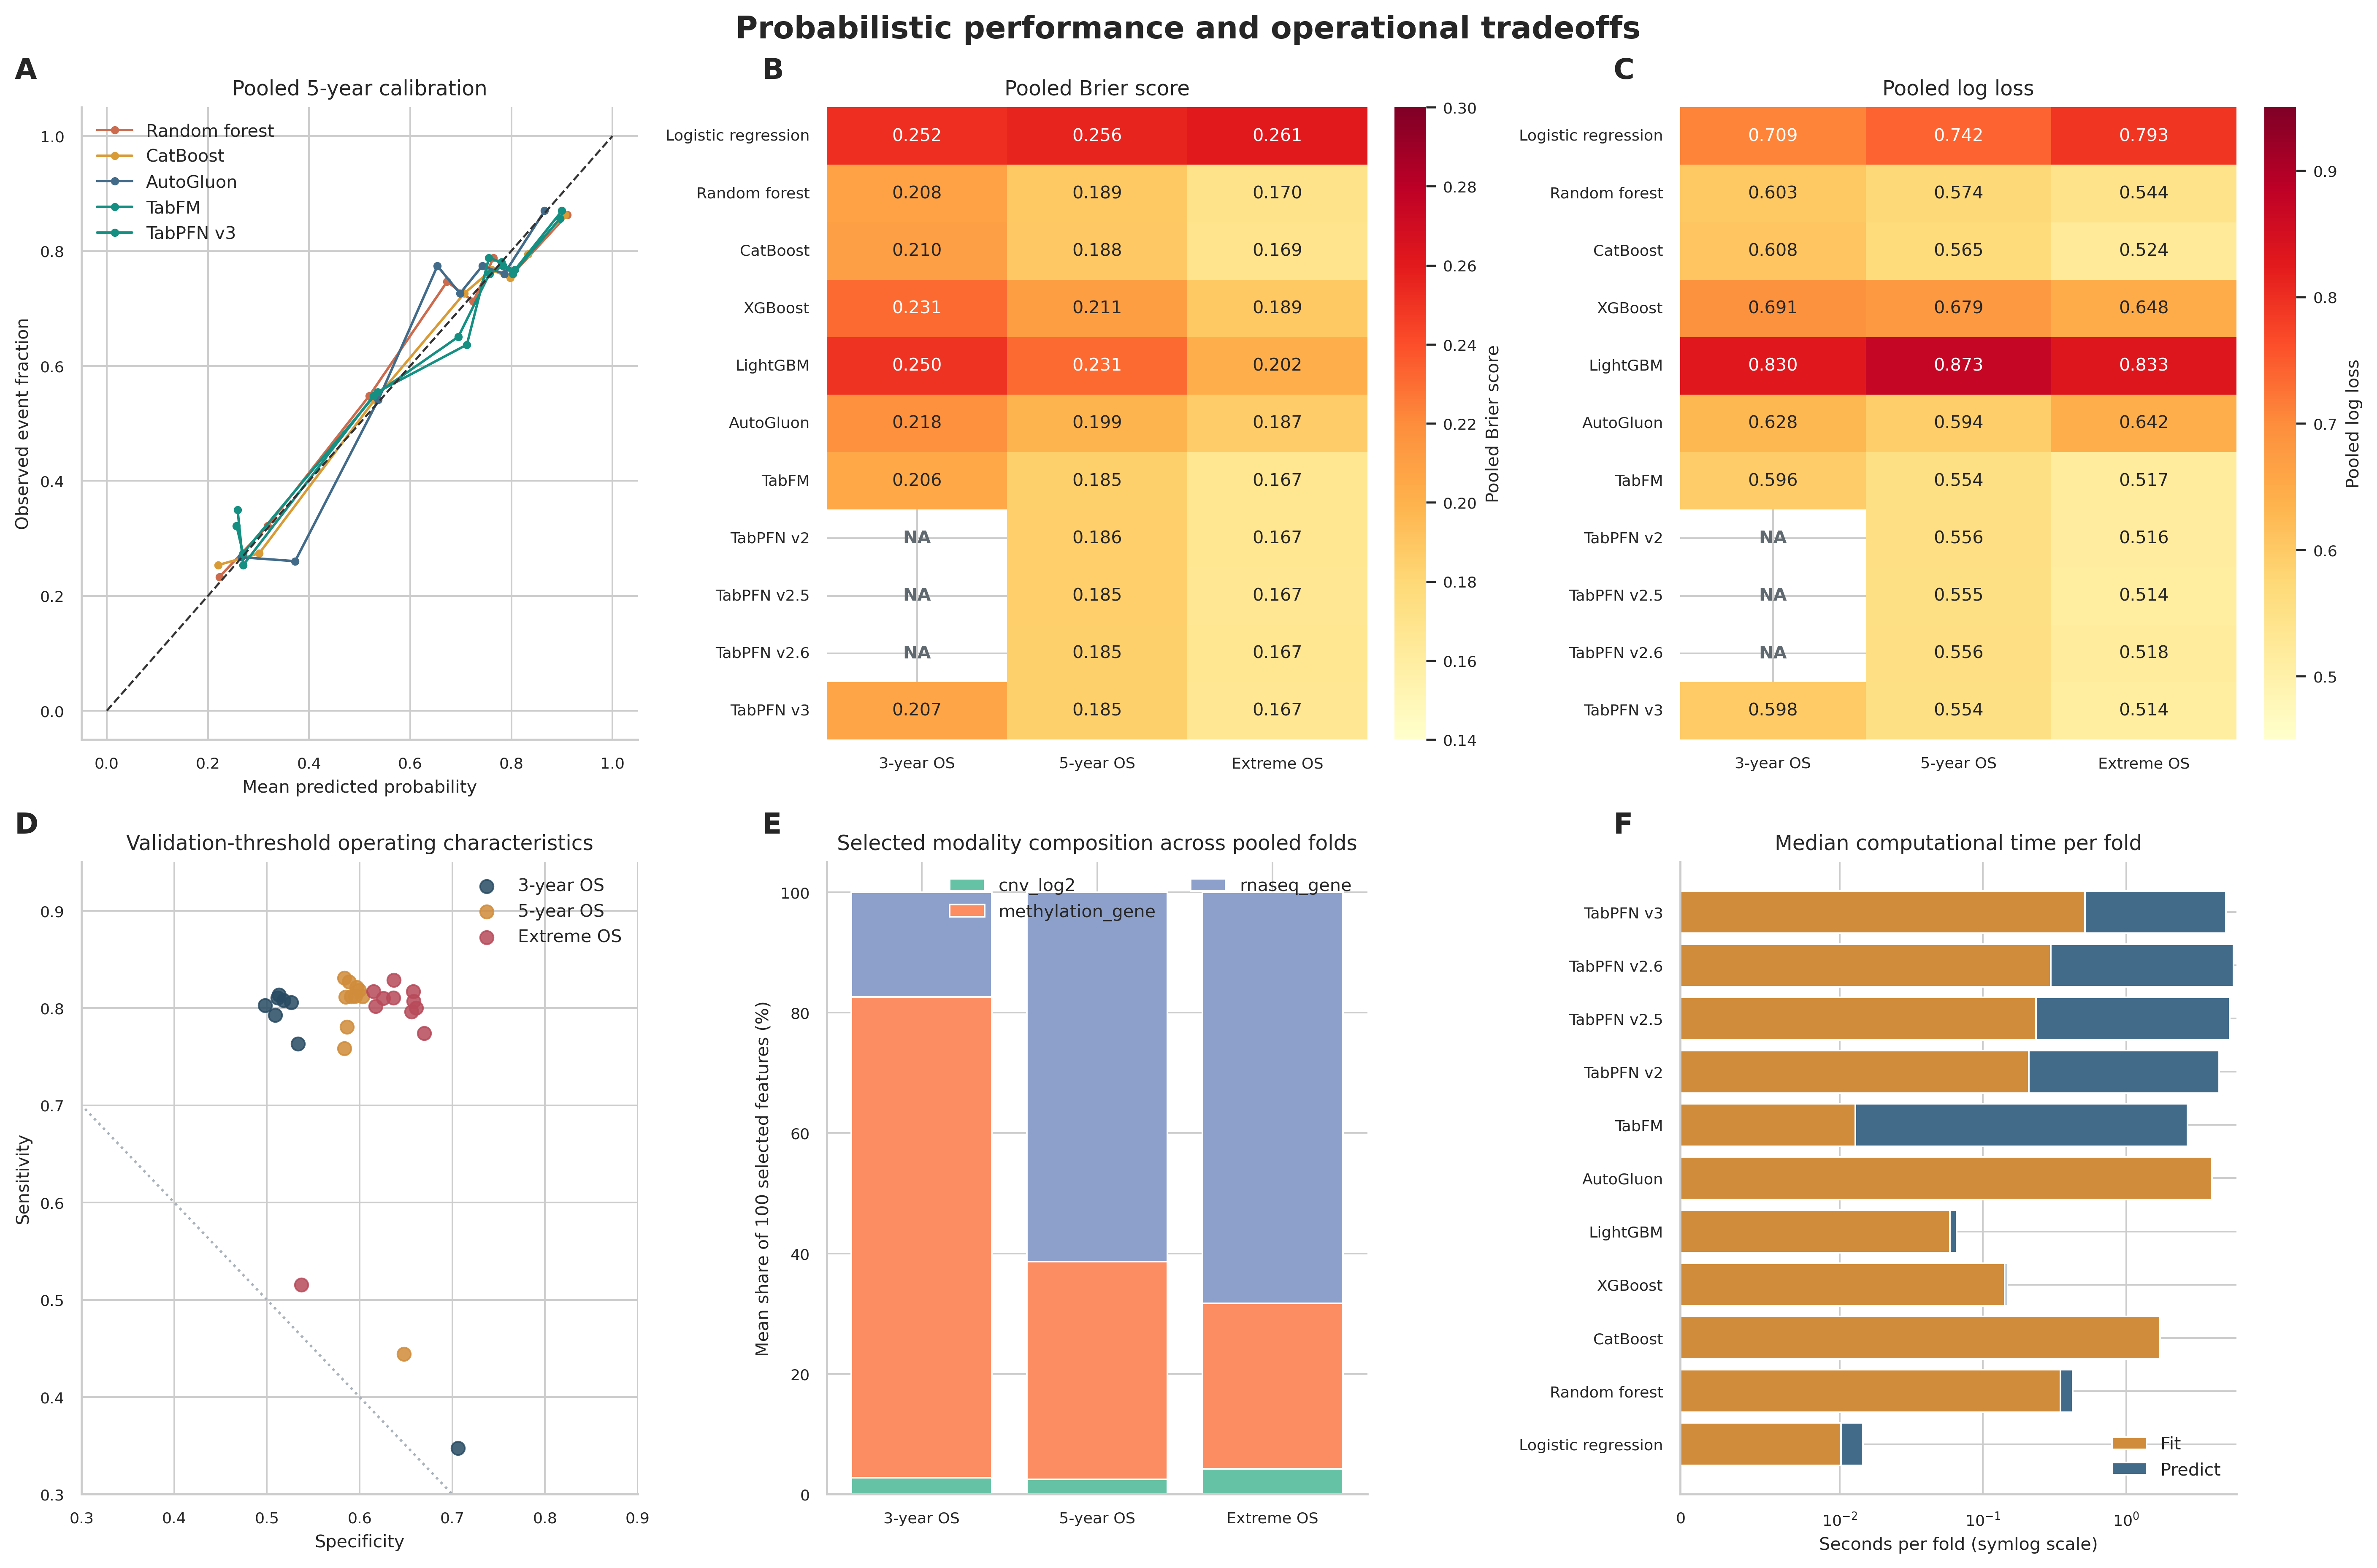
\includegraphics[width=\linewidth]{figures/manuscript/figure_05_probabilistic_and_compute.pdf}
\caption{\textbf{Probabilistic behavior, operating characteristics, feature composition, and compute.} \textbf{A}, Calibration curves for pooled 5-year predictions. \textbf{B}, pooled Brier score. \textbf{C}, pooled log loss. \textbf{D}, sensitivity and specificity at validation-selected thresholds. \textbf{E}, modality composition of features selected within training folds. \textbf{F}, median fit and prediction runtime by model. Unavailable configurations are shown as NA.}
\label{fig:probability_compute}
\end{figure}

\FloatBarrier
\section{Discussion}
\label{sec:discussion}

This study found that tabular foundation models were competitive in repeated cancer multiomics evaluation, but that the strongest visual performance gain arose from changing the evaluation population rather than from a clear architectural advantage. Within cancer cohorts, mean ROC AUC remained modest and model rankings varied across endpoints. Randomly pooling cancers produced substantially higher discrimination for foundation models, tree ensembles, and AutoML alike. The same pooled tasks, however, were predictable from cancer identity and from structural zeros introduced by cross-cohort harmonization. The central result is therefore not that foundation models recovered a general pan-cancer survival signature. It is that pooled biomedical evaluation can combine prognostic information with readily learnable cohort structure, creating scores that require cohort-aware controls before biological interpretation.

The model comparison also argues against a universal winner. TabPFN generations and TabFM occupied the upper part of the within-cancer ranking, but their advantage over random forest and CatBoost was small relative to task-level variation. AutoGluon did not dominate under its fixed budget, and classical tree models remained competitive in pooled settings. These observations are consistent with broader tabular benchmarking, where validation protocol, compute budget, and ensembling can alter rankings. They also clarify what in-context prediction contributes: reduced task-specific fitting does not remove dependence on preprocessing, context size, data distribution, or inference resources. A foundation model should therefore be evaluated as an end-to-end system rather than as a checkpoint isolated from its execution constraints.

The shortcut analyses explain why a pooled ROC AUC can rise without demonstrating shared prognostic biology. Cancer cohorts differ in baseline outcome prevalence, molecular distributions, assay coverage, and technical processing. If cancer identity can be inferred from observed values or missingness patterns, a model can partially rank survival by first locating a patient within this cohort structure. Removing an explicit cancer indicator is not sufficient because the molecular table can encode the same information indirectly. The near-perfect cancer separability obtained from structural zeros makes this mechanism especially plausible here. Cancer-held-out performance near chance further suggests that the pooled association was not robust to a shift in disease identity, although this diagnostic should not be treated as a substitute for prospective external validation.

The extreme-survival analysis illustrates a separate but related design effect. Contrasting death within 3 years against survival beyond 5 years produced the highest pooled AUCs, yet it excluded patients with intermediate trajectories and altered both prevalence and case mix. Such extreme-phenotype sampling can be valuable for mechanistic exploration because it increases separation between outcome groups, but it does not estimate performance for the original fixed-horizon population. Reporting it as a superior version of 3-year or 5-year prediction would therefore be misleading. We treat it as an exploratory estimand and interpret its stronger shortcut baselines as additional evidence that cohort composition remains influential even when outcomes are more separated.

Several limitations bound the conclusions. The analysis framed survival as fixed-horizon classification rather than modeling the full censored time-to-event distribution. Eligible sample sizes were small within several cancers, and modality availability was not uniform. The cancer-held-out and source-oriented analyses are stress tests, not a complete external validation of every model against an independently assembled clinical cohort. Probability quality was assessed through Brier score, log loss, and descriptive calibration curves, but no claim of clinical calibration or utility is made. Finally, model versions were evaluated within their available CPU execution envelopes, so cells without an evaluated configuration remain NA rather than being extrapolated or imputed.

These results suggest a practical evaluation standard for tabular foundation models in biomedicine. Models should be compared on identical patient folds with feature selection and preprocessing confined to training data. Pooled analyses should be accompanied by within-cohort estimates, prevalence-aware precision-recall summaries, cancer-only and missingness-only controls, and a cohort-held-out test. Sample-level probabilities, thresholds, model versions, runtimes, and execution hardware should be preserved. Under this standard, a high pooled score becomes one component of evidence rather than a stand-alone claim of biological generalization.

\section{Methods}
\label{sec:methods}

\subsection{Data sources and cohort definition}

The study used harmonized molecular and clinical resources representing BRCA, ESCA, HNSCC, LSCC, and LUAD. TCGA disease studies and the TCGA clinical resource provided disease definitions and outcome fields; CPTAC-derived data products contributed available proteogenomic source information.\citep{tcga2012brca,tcga2017esca,tcga2015hnsc,tcga2012lusc,tcga2014luad,liu2018clinical,li2023pancancer} Patient identifiers were used as grouping units so that multiple records from the same patient could not cross training, validation, and test partitions. The frozen fold manifest records endpoint, cohort, sample counts, split membership, selected features, and source checksums.

\subsection{Outcome definitions}

For a horizon $h$, a patient was assigned event class 1 when death was observed on or before $h$, and class 0 when follow-up extended to or beyond $h$. Patients censored before $h$ had an unknown fixed-horizon status and were excluded. Horizons were 1,095 days for 3-year survival and 1,825 days for 5-year survival. The exploratory extreme-survival endpoint contrasted death within 3 years with survival beyond 5 years. It was analyzed separately because it excludes intermediate observations and targets a different population.

\subsection{Repeated patient-grouped evaluation}

Each eligible task used five repeats of five outer folds. Within each outer fold, approximately 20\% of patients formed the test partition. The remaining patients were divided into approximately 64\% training and 16\% validation overall. Split construction was patient-grouped and class-stratified where feasible. All models used the same frozen assignments. Feature ranking was fitted on training patients only, and the 100 highest-variance eligible molecular features were retained. Validation patients were used to choose a classification threshold; test patients were not used for preprocessing, feature selection, model choice, or threshold selection.

\subsection{Models and execution}

The comparison included logistic regression, random forest, CatBoost, XGBoost, LightGBM, AutoGluon, TabFM, and TabPFN v2, v2.5, v2.6, and v3.\citep{breiman2001random,chen2016xgboost,ke2017lightgbm,prokhorenkova2018catboost,erickson2020autogluon,hollmann2025accurate,google2026tabfm,tabfmsoftware2026} Classical models were evaluated locally against the frozen fold bundles. Foundation-model and AutoGluon evaluations used CPU execution on a GCP \texttt{c3-highcpu-22} Spot instance. TabFM used the PyTorch backend, and AutoGluon used a fixed 180-second time limit per fold. Pooled 3-year entries for TabPFN v2, v2.5, and v2.6 are reported as NA because those training sets were outside the evaluated CPU row envelope. No values were imputed for unavailable configurations.

\subsection{Metrics and statistical summaries}

We retained accuracy, balanced accuracy, sensitivity, specificity, F1 score, ROC AUC, precision-recall AUC, log loss, and Brier score for each model-fold configuration. ROC AUC, precision-recall AUC, log loss, and Brier score were primary threshold-independent summaries. Sensitivity, specificity, F1 score, balanced accuracy, and accuracy used the threshold selected on the validation partition. Precision-recall AUC was interpreted relative to event prevalence. Figures report descriptive variation across repeated folds and preserve NA cells. Patient-level predictions were retained for out-of-fold ROC, precision-recall, and calibration curves. Label-permutation analyses used 500 global and 500 within-cancer permutations per endpoint, and previously generated patient-level bootstrap artifacts used 2,000 resamples.

\subsection{Shortcut and generalization diagnostics}

Cancer-identity controls estimated how much pooled outcome ranking could be obtained from cohort membership alone. Structural-zero controls used the pattern of absent or zero-filled harmonized features without relying on measured molecular magnitudes. A separate cohort-identification analysis quantified the recoverability of cancer type from these representations. Cancer-held-out linear molecular diagnostics trained on the available cancers and evaluated the omitted cancer. These analyses were interpreted as sensitivity tests for cohort dependence, not as estimates of prospective clinical performance.

\subsection{Reproducibility and reporting}

All 400 fold bundles were frozen before local or cloud model execution. Fold-level metrics, sample-level predictions, selected-feature records, manifests, software metadata, and figure source tables are retained in the project repository. Figures 1--5 were generated directly from these artifacts by \texttt{paper/analysis/build\_manuscript\_assets.py}; no simulated ROC curves, synthetic uncertainty intervals, or manually entered plotting arrays were used. Reporting was structured with reference to TRIPOD+AI and risk-of-bias considerations from PROBAST+AI.\citep{tripodai2024,probastai2024}

\section{Data and Code Availability}

The analysis code and manuscript source are available through the project repository at \url{https://github.com/HawkFranklin-Research/tab-r1}. Frozen leakage-safe fold bundles are hosted in the private Hugging Face dataset named \texttt{TABR1-Cancer-OS-LeakageSafe-Folds} under the \texttt{HawkFranklin-Research} organization. Machine-readable source data for each figure are stored under \texttt{paper/figures/source\_data}, and generated manuscript tables are stored under \texttt{paper/tables/generated}. Access to controlled or source datasets remains subject to the terms of the originating resources.

\section{Author Contributions and Disclosures}

V.P.P. conceived the study, directed the evaluation, interpreted the results, and is responsible for the manuscript. Computational tools, including language-model assistance, were used for code development, editing, and reproducibility checks under human supervision. Such tools are not authors and did not assume responsibility for the scientific conclusions. The author declares no competing interests.

\bibliography{references}

\end{document}
